\documentclass[%
  aps, reprint, prl, amsmath,amssymb
]{revtex4-2}

\usepackage{graphicx}
\graphicspath{{figures/}}
\usepackage{orcidlink}
\usepackage{mathtools}

% -------------- arXiv-Style Margin Stamp ----------------
\usepackage[style=iso]{datetime2}
\usepackage{FiraMono}
\usepackage{tikz}

\AddToHook{shipout/background}{
  \begin{tikzpicture}[remember picture, overlay]
    \node [rotate=90, color=gray!80, font=\fontfamily{FiraMono-TLF}\selectfont\footnotesize] at ([xshift=1.2cm]current page.west) {WORKING DRAFT \quad $\bullet$ \quad \DTMnow \quad $\bullet$ \quad doi.org/10.17605/OSF.IO/EV8H6 \quad $\bullet$ \quad Brian S. Mulloy \quad $\bullet$ \quad bmulloy@umich.edu};
  \end{tikzpicture}
}
% --------------------------------------------------------

\begin{document}

\title{Resolving Wigner Negativity, Semiclassical Caustics, and Schr\"{o}dinger Nodes via the Uncertainty Principle}

\begin{abstract}
Wigner negativity, semiclassical caustics, and Schr\"{o}dinger nodes follow from ignoring Heisenberg constraints --- equivalently, from assuming unbounded classical action. Enforcing the action capacity of a physical system via symplectic phase-space cells resolves all three simultaneously. The resulting phase-space densities are provably non-negative, free of turning-point divergences, and strictly positive everywhere.
\end{abstract}

\author{Brian S. Mulloy\orcidlink{0000-0002-1803-3172}}
\email{bmulloy@umich.edu}

\date{\today}

\maketitle

The WKB probability density \cite{berry1977,langer1937} diverges at every classical turning point. The Wigner--Weyl distribution \cite{wigner1932} takes negative values for any state beyond the ground state. The exact wavefunction $|\psi_n(q)|^2$ is exactly zero at every node. Each is treated as a feature of its own formalism. They share a kinematic root. Each requires evaluating a density at a point in phase space, and the uncertainty principle does not permit that. A point is a region of zero phase-space area. No physical instrument resolves zero area, and no physical state is supported there.

The matrix of pathologies and textbook remedies is small. In the semiclassical formalism, the WKB density diverges at turning points and the Airy uniform density \cite{langer1937,berry1977} is the textbook remedy: connection formulas patch the wavefunction across each turning point in an asymptotic expansion local in $q$. The patched wavefunction, Wigner-transformed, is again negative. In the wave formalism, the Wigner function goes negative under interference and the Husimi $Q$-function \cite{husimi1940} is the textbook remedy: convolution with a fixed coherent-state kernel of unit width gives a non-negative density at the cost of every scale below the ground-state cell. Schr\"odinger nodes \cite{robertson1929,schrodinger1930} are exact zeros of the wavefunction. They have no textbook remedy and are read as a structural feature of the spectrum. None of the three remedies addresses the others.

The three pathologies dissolve together when the question is asked at the resolution physics permits. The smallest cell of phase space that admits a physical answer has area $h/2$. Inside any larger cell, the conjugate substructure has reciprocal widths $\delta q = \hbar/\Delta p$ and $\delta p = \hbar/\Delta q$ \cite{zurek2001}. The minimum area cannot be evaded by squeezing along any conjugate axis pair \cite{gromov1985}. Together these fix a unique pair of squeezed Gaussian kernels of phase-space area $h/2$ at every point in the orbit's covariance ellipse. The convolution of any quantum or classical phase-space density with such a kernel is non-negative \cite{hudson1974} and finite. The same kinematic constraint that rules out pointwise infinity rules out pointwise zero, so the resolved density is strictly positive throughout phase space.

\begin{figure}[t]
\centering
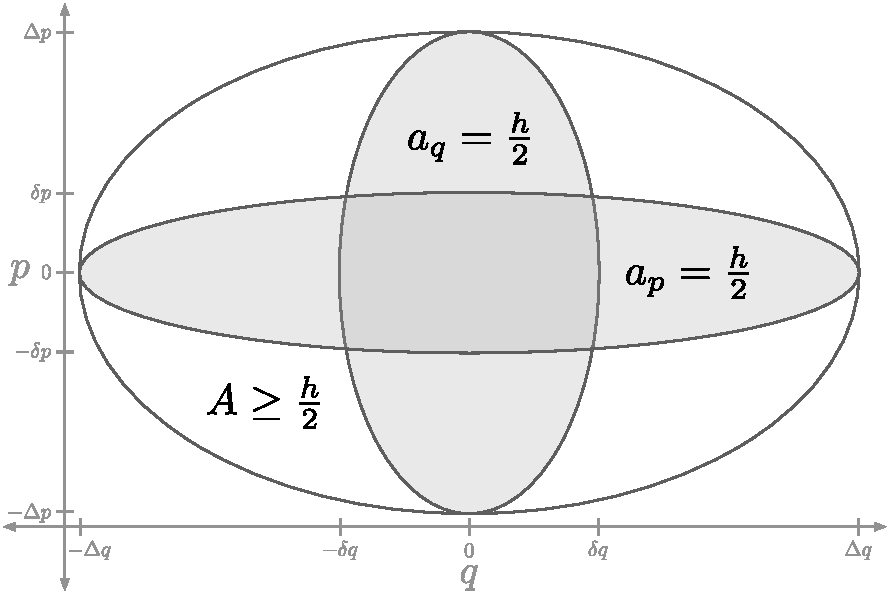
\includegraphics[width=\linewidth]{figures/quantum_of_action.pdf}
\caption{\textbf{The symplectic quantum of action} (schematic, 1D case). The Heisenberg limit $\sigma_q \sigma_p \ge \hbar/2$ admits classical semi-axes $\Delta q = \sqrt{2}\sigma_q$, $\Delta p = \sqrt{2}\sigma_p$; the $1\sigma$ contour of the state's covariance projects onto a Fermi blob \cite{degosson2012fermi} of phase-space area $A = \pi \Delta q \Delta p \ge h/2$. Inside the blob sit a conjugate pair of orthogonal quantum blobs, $a_q = \pi\,\delta q\,\Delta p = h/2$ and $a_p = \pi\,\Delta q\,\delta p = h/2$, summing to the quantum of action $h = a_q + a_p$. Their minor semi-axes are the reciprocal scales $\delta q = \hbar/\Delta p$ and $\delta p = \hbar/\Delta q$; $a_q$ is squeezed along position, $a_p$ along momentum. As $A$ grows, $a_q$ and $a_p$ compress along their conjugate axes and phase-space resolution sharpens.}
\label{fig:quantum_of_action}
\end{figure}

The Fermi blob \cite{degosson2012fermi} of an energy eigenstate sits on the classical orbit at the Bohr--Sommerfeld energy $E_n$. The orbit's time-averaged second moments give classical semi-axes $\Delta q = \sqrt{2\langle (q-\langle q\rangle)^2\rangle_\text{orbit}}$ and $\Delta p = \sqrt{2\langle p^2\rangle_\text{orbit}}$, and the blob has area
\begin{equation}
A = \pi \Delta q \Delta p \ge \frac{h}{2}.
\label{eq:fermi_blob_area}
\end{equation}
The Heisenberg limit imposes $A \ge h/2$, with the lower bound saturated by minimum-uncertainty Gaussians. The Robertson--Schr\"odinger inequality \cite{robertson1929,schrodinger1930} is the constraint these moments respect, not their source. The reciprocal scales partition the blob's interior; the conjugate quantum blobs \cite{degosson2009,degossoncharlyne2022},
\begin{equation}
a_q = \pi\,\delta q\,\Delta p = \frac{h}{2}, \qquad a_p = \pi\,\Delta q\,\delta p = \frac{h}{2},
\end{equation}
each carry the irreducible area $h/2$, $a_q$ squeezed along the position axis, $a_p$ along the momentum axis (Fig.~\ref{fig:quantum_of_action}). A non-eigenstate has no orbit; its moments come from the Robertson--Schr\"odinger covariance of the state directly.

The action capacity $A$ and the Bohr--Sommerfeld action $A_\text{BS} = \oint p\, dq$ are different objects. Both have units of action; they describe different geometric content. For the harmonic oscillator they coincide and the Fermi blob equals the energy-shell ellipse. For anharmonic potentials they separate, with $A \le A_\text{BS}$. The kernel widths $\delta q$ and $\delta p$ track $A$, the orbit's covariance, not $A_\text{BS}$, the area it encloses.

The kernels of phase-space area $h/2$ corresponding to the conjugate quantum blobs are
\begin{equation}
G_{\delta q}(q,p) = \frac{1}{\pi}\exp\!\left(-\frac{q^2}{\delta q^2} - \frac{p^2}{\Delta p^2}\right),
\end{equation}
\begin{equation}
G_{\delta p}(q,p) = \frac{1}{\pi}\exp\!\left(-\frac{q^2}{\Delta q^2} - \frac{p^2}{\delta p^2}\right).
\end{equation}
$G_{\delta q}$ is squeezed along the position axis and spans $\Delta p$ in momentum; $G_{\delta p}$ is the conjugate. Each saturates the symplectic-capacity bound at $h/2$. The same kernel, fixed by the orbit, applies to two distinct inputs. For the classical microcanonical density $W_\text{cl}(q,p) \propto \delta(H - E)$, the marginal of the convolution over $p$ is
\begin{equation}
\rho_{\delta q}(q) = \int (W_\text{cl} * G_{\delta q})(q,p)\, dp,
\label{eq:rho_marginal}
\end{equation}
finite even where $P_\text{WKB}$ diverges. For the quantum Wigner function the convolved phase-space density is
\begin{equation}
P_{\delta q}(q,p) = (W * G_{\delta q})(q,p),
\end{equation}
non-negative everywhere because the kernel attains the symplectic positivity condition \cite{hudson1974}. The kernel's Gaussian tails are everywhere positive, so both convolutions are everywhere strictly positive --- a fact that returns when tunneling appears in the double-well barrier interior.

\begin{figure}[!htbp]
\centering
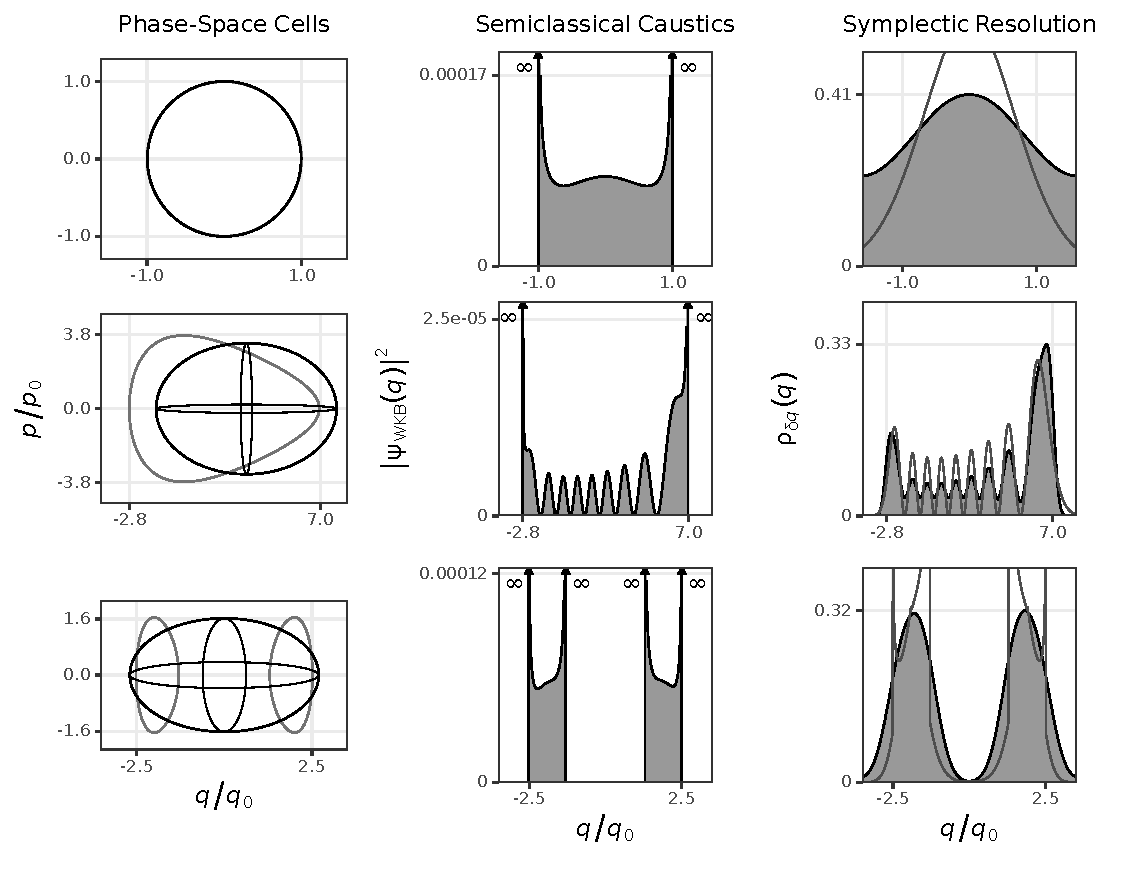
\includegraphics[width=\linewidth]{figures/semiclassical.pdf}
\caption{\textbf{Semiclassical resolution.} Rows show the harmonic ground state, Morse $n = 8$, and the symmetric double-well sub-barrier doublet at action capacity $A_\text{BS}/A_0 \approx 1.976$. \textit{Left:} Classical orbit at $E_n$ with the symplectic quantum of action overlaid. \textit{Center:} Oscillating WKB density $|\psi_\text{WKB}(q)|^2 = (A^2/p)\cos^2(S/\hbar - \pi/4)$ with caustic divergences (rendered as infinity arrows) at every classical turning point. The double-well row has four divergences, two per well. \textit{Right:} Resolved density $\rho_{\delta q}(q)$ with the per-orbit Airy uniform density \cite{langer1937} overlaid. The harmonic row reduces to a single Gaussian. The Morse row preserves the $n+1$ WKB lobes; the divergences become finite peaks. The double-well row resolves the two-well structure smoothly. Per-well Airy lobe maxima clip the panel at every inner turning point --- standard behavior of the Airy uniform density at a sub-barrier well boundary, displayed honestly; the resolved density is everywhere finite.}
\label{fig:semiclassical}
\end{figure}

\begin{figure}[!htbp]
\centering
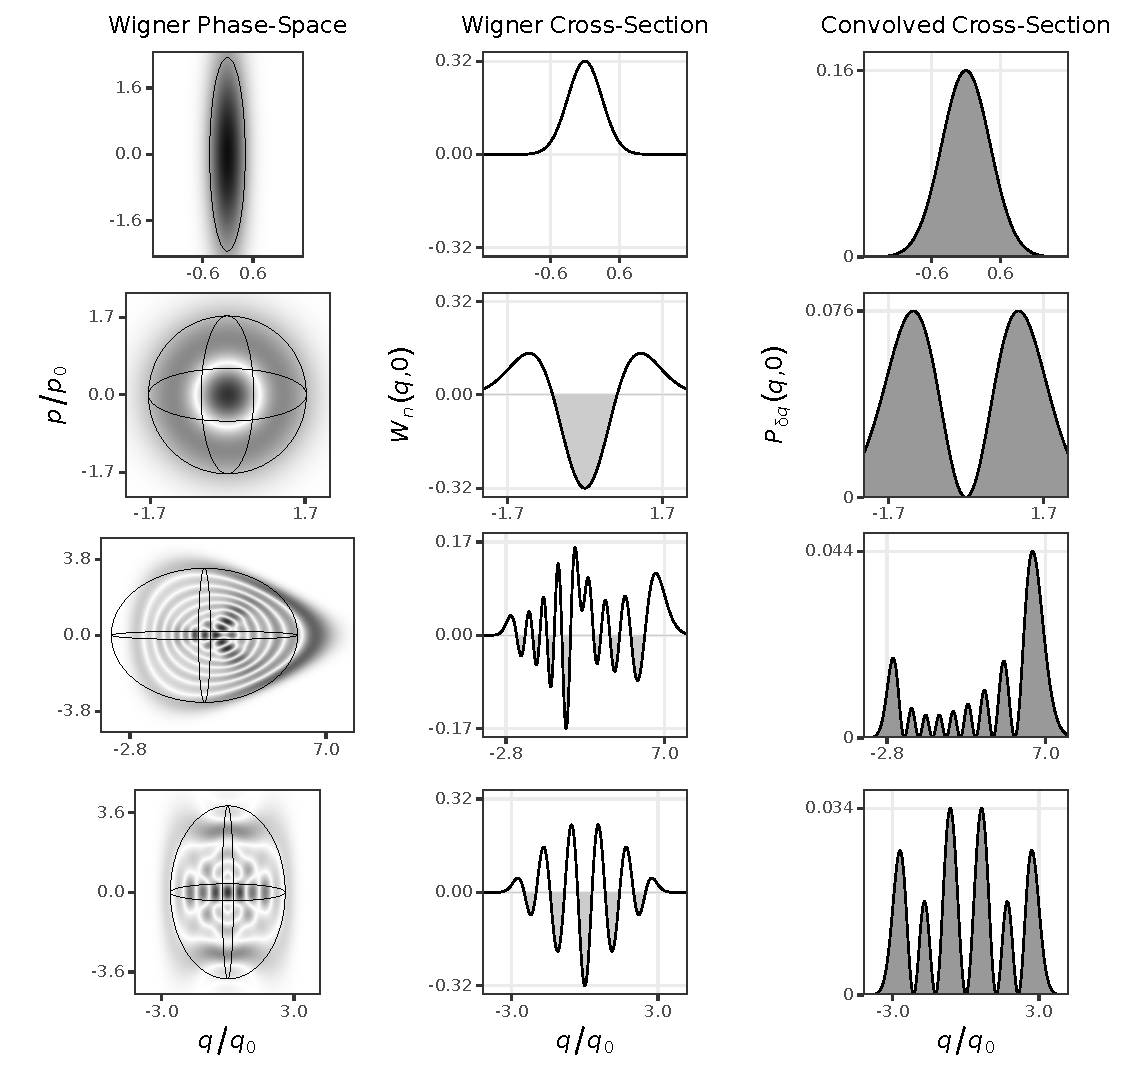
\includegraphics[width=\linewidth]{figures/wigner.pdf}
\caption{\textbf{Wigner resolution.} Same three systems as Fig.~\ref{fig:semiclassical}, evaluated as Schr\"odinger eigenstates: harmonic $n=0$, Morse $n=8$, double-well $n=1$ (antisymmetric lower-doublet partner with exact node $\psi_1(0) = 0$). Kernel widths from the Robertson--Schr\"odinger covariance of $\psi_n$. \textit{Left:} Wigner distribution $W_n(q,p)$ with the symplectic quantum of action overlaid. \textit{Center:} Cross-section $W_n(q,0)$. The double-well row reaches $W_1(0,0) = -0.32$; the wavefunction's exact node lies at the deepest point of the Wigner negativity. \textit{Right:} Cross-section $P_{\delta q}(q,0)$ with the Husimi cross-section $Q(q,0)$ overlaid. The Husimi kernel of width $q_0 = 1$ exceeds $\delta q$ for the Morse row and collapses the multi-lobe structure into a single peak; $\delta q$ tracks the wavefunction and resolves the lobes. At the double-well node the resolved density is strictly positive (numerically $5\times 10^{-6}$ relative to peak $\sim 0.08$); the two pathologies that the title's figure exhibits --- Wigner negativity and Schr\"odinger nodes --- resolve at the same kernel.}
\label{fig:wigner}
\end{figure}

For the Morse oscillator $V(q) = D_e(1 - e^{-\alpha q})^2$ with $D_e = 12.5$, $\alpha = 0.2$, $m = 1$, the natural frequency $\omega_0 = \alpha\sqrt{2D_e/m} = 1$. Bound states have $A < A_\text{BS}$, with the gap widening as the orbit reaches into the soft-wall region. Figure~\ref{fig:semiclassical} shows the semiclassical pipeline at three action capacities. The harmonic ground state ($A_\text{BS}/A_0 = 1$) is the floor: the WKB density is a single $\cos^2$ lobe with caustic divergences at the two turning points; the resolved density is a single Gaussian; Airy and the resolved density agree. The Morse row at $n = 8$ carries the canonical Bohr--Sommerfeld interference --- the half-orbit phase advances by $\pi(n + 1/2)$ and $\cos^2$ of that phase has $n$ zeros and $n+1$ peaks --- together with caustic divergences at the two turning points. At resolution $\delta q$, the divergences become finite peaks; the lobe envelope persists. Airy agrees on lobe count and envelope but has taller peaks and zero troughs because Airy is evaluated at infinite resolution. The double-well row sits at the lowest sub-barrier doublet, $A_\text{BS}/A_0 \approx 1.976$ (chosen to align with Schr\"odinger $n=1$ at $E = -2.652$). Two disconnected classical loops, four turning points, four caustic divergences. The per-well Langer--Airy construction places lobe maxima at every inner turning point and clips the panel; the resolved density is everywhere finite and resolves the two-well structure smoothly. Higher-order uniform constructions exist for sub-barrier doublet topology (parabolic-cylinder matching across the barrier; Mathieu-function uniform approximations) but require state-specific machinery beyond Langer's universal turning-point patch; per-well Langer is the textbook prior art and we display it as such.

The same kinematic root rules out pointwise infinity and pointwise zero. A density at the value $\infty$ requires concentrating finite probability into zero width: $\delta q \to 0$, hence $\Delta p \to \infty$, hence unbounded action. A density at the value $0$ requires resolving the field to a single point: $\delta q \to 0$ again, hence the same unbounded action. The exact zeros of $|\psi_n(q)|^2$ at the wavefunction's nodes are the reciprocal of the WKB infinity at the turning points. Neither survives at any finite resolution. Figure~\ref{fig:wigner} shows the three systems in the wave formalism, with kernel widths now from the Robertson--Schr\"odinger covariance of $\psi_n$ rather than the classical orbit. The Morse row at $n = 8$ develops $n+1$ alternating-sign lobes whose envelope tracks the asymmetric orbit; at resolution $\delta q$ the cross-section is non-negative \cite{hudson1974} and the lobe envelope persists. Husimi, with its fixed kernel of width $q_0 = 1$, smooths the envelope into a single peak; the contrast grows with $n$ as $\delta q/q_0$ shrinks. The double-well antisymmetric partner $\psi_1$ has a node at $q=0$, an exact zero of $|\psi_1|^2$; the same point is the deepest Wigner negativity, $W_1(0,0) = -\Delta E$ at the doublet scale. At resolution $\delta q$ the resolved density is strictly positive throughout, including across the node and through the barrier. The classical microcanonical density has no support in the barrier, but the kernel's Gaussian tails extend across it from each well, so the resolved density is exponentially small but nonzero throughout the barrier interior. The inter-well coupling that conventional treatments add by hand is what the cell physics, asked the right question, reports.

\begin{figure}[!htbp]
\centering
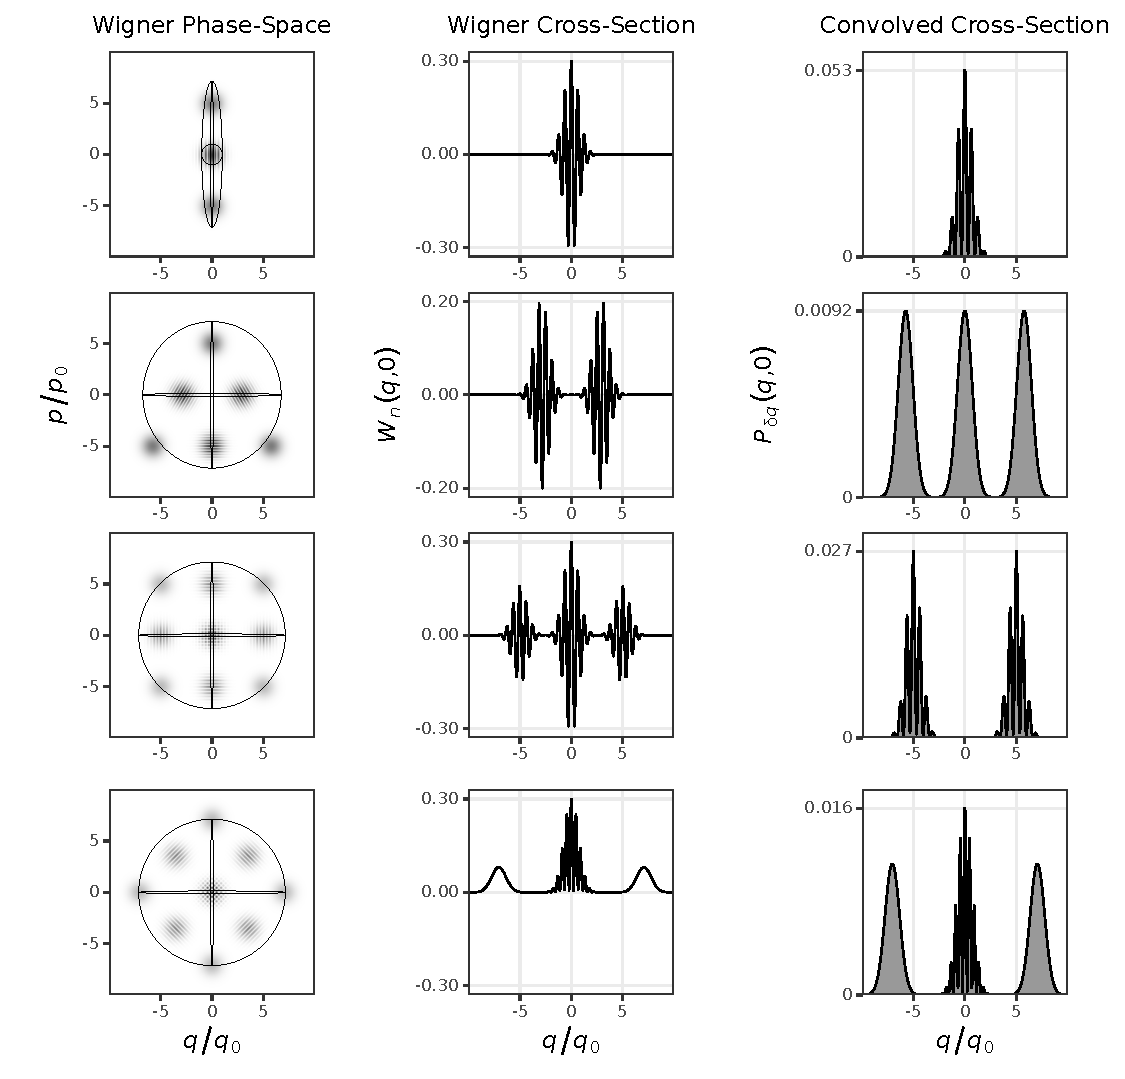
\includegraphics[width=\linewidth]{figures/cats.pdf}
\caption{\textbf{Cat states.} Coherent superpositions of $n$ Gaussian wavepackets with no classical orbit and no Bohr--Sommerfeld condition. Kernel widths from the Robertson--Schr\"odinger covariance of $\psi$ directly. Rows: 2-cat at $(0, \pm 5)$; 3-cat at the equilateral triangle apex $(0,5)$ and base $(\pm 10/\sqrt{3}, -5)$; 4-cat compass at $(\pm 5, 0), (0, \pm 5)$ \cite{zurek2001}; 4-cat compass rotated $45^\circ$ to the diagonals $(\pm 5, \pm 5)$. Columns as in Fig.~\ref{fig:wigner}. Each row's Wigner cross-section dips below zero --- the central interference fringe of the 2-cat, the pair-fringe envelopes of the 3-cat, the on-slice lobes plus chessboard of the axis-aligned compass, the off-slice midpoint fringes plus sub-Planck chessboard \cite{zurek2001} of the rotated compass. The resolved density $P_{\delta q}(q,0)$ is non-negative for every row. The two compass orientations carry the same number of lobes; rotation moves their projections onto the $p=0$ slice and changes what the cross-section sees while the kernel does its job either way.}
\label{fig:cats}
\end{figure}

Cat states have no orbit. The construction's widths come from the orbit when one exists; for non-eigenstates they come from the Robertson--Schr\"odinger covariance of the wavefunction directly --- the same scalar quantities, $\Delta q = \sqrt{2\sigma_{qq}}$, $\Delta p = \sqrt{2\sigma_{pp}}$, computed from $\langle q^2\rangle_\psi$ and $\langle p^2\rangle_\psi$ instead of the orbit's time-average. Figure~\ref{fig:cats} shows the construction applied to four cat configurations \cite{schleich2001}. Each row's Wigner has lobe Gaussians at the cat positions and oscillating cross-fringe envelopes at every pair midpoint; the cross-section $W(q,0)$ at $p=0$ shows whatever content lies on that slice. The 2-cat slice sees the central interference fringe between two lobes that sit off the slice; the 3-cat slice sees two pair-fringe envelopes; the axis-aligned 4-cat slice sees two lobes directly and the central chessboard \cite{zurek2001} where two diagonal pair-midpoints overlap; the rotated 4-cat slice sees four edge-midpoint pair-fringe envelopes and the same chessboard at the origin. At resolution $\delta q$ every cross-section becomes non-negative. The two compass orientations have the same lobe count and the same total action capacity; rotation changes only the lobe positions, and so changes what the $p=0$ slice projects, while the kernel's positivity holds.

The construction has no free parameters. $\Delta q$ and $\Delta p$ come from the orbit when an orbit exists or from the wavefunction's covariance when it does not; $\delta q$ and $\delta p$ from the reciprocal scales; the kernel from the Heisenberg limit. Wigner negativity, semiclassical caustics, and Schr\"odinger nodes are not three pathologies of three formalisms. They are three artifacts of one unphysical assumption, and they go away when the assumption goes.

\medskip
All numerical data, figure-generating code, and reproducibility scaffolding for this paper are available at \url{https://doi.org/10.17605/OSF.IO/EV8H6}.

\bibliography{main}

\end{document}
